\subsection{Modes in Waveguides}\label{sec:modes_tem_cell}
\subsubsection{Rectangular Waveguides as non-TEM structures}

\begin{figure}[htbp]
	\centering
	\begin{subfigure}[b]{0.45\textwidth}
			\centering
		\includegraphics[width=1\linewidth]{content/img/rect_waveguide_tm}
		\caption{TM\textsubscript{11} mode}
		\label{fig:rectwaveguidetm}
	\end{subfigure}
	\hfill
	\begin{subfigure}[b]{0.45\textwidth}
	\centering
\includegraphics[width=1\linewidth]{content/img/rect_waveguide_te}
\caption{TE\textsubscript{10} mode}
\label{fig:rectwaveguidete}
	\end{subfigure}
	
	\caption{The electric and magnetic fields corresponding to the first dominant TE and TM modes in a rectangular waveguide with perfectly conducting walls.}
	\label{fig:rect_waveguide_modes}
\end{figure}


Waveguides with perfectly conducting walls preclude the propagation of TEM modes. In rectangular waveguides, the allowable solutions to the wave equation are restricted to TE and TM modes. The field distributions for the two primary dominant modes are depicted in \autoref{fig:rect_waveguide_modes}. 

The physical impossibility of TEM propagation within these structures is a direct 
consequence of Maxwell’s equations. Following the analytical framework established 
in \cite[pp.~425-427]{Griffiths_2024}, we demonstrate this by first decomposing 
the electric field intensity $\mathbf{E}$ and magnetic field intensity $\mathbf{H}$ 
into their longitudinal and transverse components, assuming wave propagation 
in the $z$-direction::

\begin{subequations}
	\begin{align}
		\mathbf{E}&=(E_{x}\cdot\mathbf{\hat{a}}_x+E_{y}\cdot\mathbf{\hat{a}}_y+E_{z}\cdot\mathbf{\hat{a}}_z)\mathrm{e}^{-jkz},\label{eqn:rect_e}\\
		\mathbf{H}&=(H_{x}\cdot\mathbf{\hat{a}}_x+H_{y}\cdot\mathbf{\hat{a}}_y+H_{z}\cdot\mathbf{\hat{a}}_z)\mathrm{e}^{-jkz}.\label{eqn:rect_h}
	\end{align}
\end{subequations}

Next, applying Faraday's and Ampère-Maxwell law to (\ref{eqn:rect_e}) and (\ref{eqn:rect_h}) yields \cite[p.~426]{Griffiths_2024}

\begin{subequations}
\begin{align}
	\nabla \times \mathbf{E} &=\begin{pmatrix}\frac{\partial}{\partial y}E_z-jkE_y \\jkE_x-\frac{\partial}{\partial x}E_z \\\frac{\partial}{\partial x}E_y-\frac{\partial}{\partial y}E_x\end{pmatrix}=\begin{pmatrix} -j\omega B_x\\-j\omega B_y\\ -j\omega B_z \end{pmatrix},\label{eqn:faraday}\\
	\nabla \times \mathbf{B} &=\begin{pmatrix}\frac{\partial}{\partial y}B_z-jkB_y \\jkB_x-\frac{\partial}{\partial x}B_z \\\frac{\partial}{\partial x}B_y-\frac{\partial}{\partial y}B_x\end{pmatrix}=\begin{pmatrix} \frac{j\omega}{\mu\epsilon} E_x\\\frac{j\omega}{\mu\epsilon} E_y\\ \frac{j\omega}{\mu\epsilon} E_z \end{pmatrix}.\label{eqn:ampere_maxwell}
\end{align}
\end{subequations}

For a TEM mode, the longitudinal field components vanish $E_\mathrm{z}=H_\mathrm{z}=0$. Consequently, \ref{eqn:faraday}) and (\ref{eqn:ampere_maxwell}) reduce to the following conditions for the transverse electric field components:

\begin{align}
	\frac{\partial}{\partial x}E_x+\frac{\partial}{\partial y}E_y&=0\quad\text{Derived from Gauss' law}\label{eqn:rect_waveguide_gauss},\\
	\frac{\partial}{\partial y}E_x-\frac{\partial}{\partial x}E_y&=0\quad\text{Derived from Faraday's law}\label{eqn:rect_waveguide_faraday}.
\end{align}

Since the solutions in \crefrange{eqn:rect_waveguide_gauss}{eqn:rect_waveguide_faraday} cannot satisfy the rectangular waveguide's boundary conditions, a TEM mode cannot propagate.

\subsection[TEM mode in the TEM cell]{TEM mode in the TEM cell\protect\footnote{This chapter is based on and contains significant excerpts from: P. F. Wilson et al., \textit{Excitation of a TEM cell by a Vertical Electric Hertzian Dipole}, National Bureau of Standards, 1981}}\label{sec:tem_mode_tem_cell}

In contrast to the rectangular waveguide, a TEM cell supports the propagation of TEM waves. Moreover, the TEM mode is inherently excited by the geometry of the TEM cell, and is therefore referred to as the essential mode. Higher-order TE and TM modes, which arise only due to non-uniformities in the TEM cell, are termed non-essential modes \cite{990711}.

The TEM mode in the TEM cell is derived using a procedure presented in \cites{Tippet_Chang_Crawford_1976,Wilson_1981}. This approach involves determining the Green's function for the longitudinal field components, $H_z$ and $E_z$, of both the TE and TM modes in a rectangular waveguide. The Green's function satisfies the wave equations and boundary conditions of the waveguide, and is constructed as described in \cref{sec:scal_green}, with

\begin{subequations}
	
	\begin{equation}
		(\nabla^2 + k_{t}^2) G_j (\mathbf{x}_t, \mathbf{x}_t') = -\delta(\mathbf{x}_t - \mathbf{x}_t'),
	\end{equation}
	
	\begin{equation}
		\frac{\partial G_j(\mathbf{x}_t, \mathbf{x}_t')}{\partial n}=0.
		\label{eqn:bc_tem} 
	\end{equation}

\end{subequations}

The wave number is separated into transverse and longitudinal components, $k^2 = k_{t}^2 + k_{z}^2$. Equation (\ref{eqn:bc_tem}) specifies the boundary conditions on the perfectly conducting walls and septum of the TEM cell, as well as on the gaps, as illustrated in \autoref{fig:greentemcell}. The index $j$ indicates the chamber to which the Green's function applies ($j=1$ for the upper chamber, $j=2$ for the lower chamber). The source points are denoted by $\mathbf{x'}_t = (\mathbf{\hat{a}}_x x' + \mathbf{\hat{a}}_y y')$, and the observation points by $\mathbf{x}_t = (\mathbf{\hat{a}}_x x + \mathbf{\hat{a}}_y y)$. These coordinates are transformed to depend on the wave number $k$ instead of the $z$-coordinate, which significantly simplifies the derivation of the Green's function, as only a two-dimensional surface must be considered.

\begin{figure}[bt]
	\centering
	\includegraphics[width=0.7\linewidth]{content/img/green_tem_cell}
	\caption{In this analysis, the Green's function determines the fields within the cross-sectional surface $S$ of the TEM cell, which is shown in light gray and bounded by $l$. The source exciting these fields is a centrally located electric dipole moment, $\mathbf{m}_e$.}
	\label{fig:greentemcell}
\end{figure}

The waveguide is excited by an infinitesimal electric dipole moment, centrally located and oriented along the $y$-axis. Solving for $H_z$ and applying Green’s second identity yields \cite[p.~5]{Wilson_1981}

\begin{align}
	\int_l \left( G_j(\mathbf{x}_t, \mathbf{x}_t') \frac{\partial H_z(\mathbf{x}_t)}{\partial n} - H_z(\mathbf{x'}_t){\frac{\partial G_j(\mathbf{x}_t, \mathbf{x}_t')}{\partial n}}\right)\,&d\mathbf{l'} =\\ = H_z(\mathbf{x}_t)-\int_S G_j(\mathbf{x}_t, \mathbf{x}_t') \frac{\partial J_y(\mathbf{x'}_t)}{\partial x'}\,&d\mathbf{s}',
	\label{eqn:second_green}
\end{align}

Here, $S$ denotes the waveguide cross-section and $l$ its boundary. Applying the boundary condition (\ref{eqn:bc_tem}) to the perfectly conducting septum and walls reduces the boundary integrals to those over the gaps. The electric dipole is then substituted into \eqref{eqn:second_green}, and continuity of $H_z$ and $\partial H_z / \partial y$ across these gaps is enforced. The normal vector in the gap region is oriented along the $y$-direction, $n = \pm y$. Accordingly, the line element in the integrand becomes $d\mathbf{l}' = dx'$. The right-hand side of \eqref{eqn:second_green} is integrated by parts. Finally, assuming that the electric dipole moment is located in the upper chamber, only $G_1$ needs to be considered. For the boundary, $G(x,x') = G_1(x,0,x',0) + G_2(x,0,x',0)$. Altogether, this yields \cite[pp.~5--6]{Wilson_1981}

 \begin{equation}
 		\int_\mathrm{gaps} G(x, x') \frac{\partial H_z(x',0)}{\partial y'}\,dx' = -\mathbf{m}_e \frac{\partial G_1(x,0, \mathbf{x}_t')}{\partial x'}.
 \end{equation}

Solving for the Green's function $G$ provides a solution for the longitudinal 
magnetic field intensity $H_z$ of the TE mode. An analogous procedure can be 
used to determine the longitudinal electric field intensity $E_z$ of the TM mode. 
As shown in \cite{Wilson_1981}, the total field distribution is then given by the 
superposition of the TE and TM mode fields, thereby demonstrating the excitation 
of the TEM mode. The transverse fields $\mathbf{E}_t$ and $\mathbf{H}_t$ can then 
be derived from the longitudinal field components $H_z$ and $E_z$. They are 
related to $H_z$ by \cite[p.~3]{Wilson_1981}
\begin{subequations}
	\begin{equation}
		\mathbf{E}_t(\mathbf{x}_t) = \frac{j\omega\mu_0}{k_{t}^2}\, \nabla_t H_z(\mathbf{x}_t) \times \hat{\mathbf{a}}_z,
	\end{equation}
	\begin{equation}
		\mathbf{H}_t(\mathbf{x}_t) = -\frac{j k_{z}}{k_{t}^2}\, \nabla_t H_z(\mathbf{x}_t),
	\end{equation}
\end{subequations}
and to $E_z$ by
\begin{subequations}
	\begin{equation}
		\mathbf{E}_t(\mathbf{x}_t) = -\frac{j k_{z}}{k_{t}^2}\,\nabla_t E_z(\mathbf{x}_t),
	\end{equation}
	\begin{equation}
		\mathbf{H}_t(\mathbf{x}_t) = \frac{-j\omega\epsilon_0}{k_{t}^2}\, \nabla_t E_z(\mathbf{x}_t) \times \hat{\mathbf{a}}_z,
	\end{equation}
\end{subequations}
where $\nabla_t=\partial/\partial x + \partial/\partial y$ denotes the transverse gradient operator.

\subsubsection{Higher-order modes}\label{sec:higher-order-modes}

To determine the usable frequency range of the TEM cell shown in 
\autoref{fig:tem_cell_model2}, the cutoff frequencies of its higher-order modes are 
examined. Among these, the TE\textsubscript{10} and TE\textsubscript{01} modes are of primary interest as they exhibit the lowest cutoff frequencies. Their transverse electric field distributions are illustrated in \autoref{fig:transversal_e_fields_tem_cell}, while \autoref{fig:waveguide-modes} shows the electric and magnetic field distributions along the TEM cell for each mode. As visible there, the TEM mode exhibits the highest phase velocity, reflected in the large number of periods along the cell, and its magnetic field has no longitudinal component. In contrast, the TE\textsubscript{01} and TE\textsubscript{10} modes possess longitudinal magnetic field components. For the 
TE\textsubscript{01} mode, these are concentrated near the side walls and are therefore not directly shown in \autoref{fig:waveguide-modes}.
\begin{figure}[h]
	\centering
	\begin{subfigure}[b]{0.3\linewidth}
		\centering
		\includegraphics[width=\linewidth]{content/img/tem_cell_mode.png}
		\caption{TEM mode}
		\label{fig:tem_mode}
	\end{subfigure}
	\begin{subfigure}[b]{0.3\linewidth}
		\centering
		\includegraphics[width=\linewidth]{content/img/te01_mode.png}
		\caption{TE\textsubscript{01} mode}
		\label{fig:te01_mode}
	\end{subfigure}
	\begin{subfigure}[b]{0.3\linewidth}
		\centering
		\includegraphics[width=\linewidth]{content/img/te10_mode.png}
		\caption{TE\textsubscript{10} mode}
		\label{fig:te10_mode}
	\end{subfigure}
	\caption{Transverse electric field distributions in the cross section of the TEM cell.}
	\label{fig:transversal_e_fields_tem_cell}
\end{figure}
For a thin septum ($t/b \ll 0.1$), the cutoff frequencies of modes with even $n$ 
subscripts, i.e. TE\textsubscript{m,2n} and TM\textsubscript{m,2n} modes, can be 
approximated by the cutoff frequency expression for rectangular waveguides 
\cite{Weil_Gruner_1984}
\begin{equation}
	f_c = \frac{c}{2} \sqrt{\left(\frac{m}{a}\right)^2 + \left(\frac{n}{b}\right)^2},
	\label{eqn:cutoff_frequency_rect_waveguide}
\end{equation}
where $c$ is the speed of light, and $m \geq 0$ and $n \geq 0$ are the integer mode 
indices along the $a$- and $b$-directions, respectively. Applying 
\eqref{eqn:cutoff_frequency_rect_waveguide} to a TEM cell with $a=40\,\mathrm{mm}$, 
$b=24\,\mathrm{mm}$, $g=5\,\mathrm{mm}$, and $t=0.1\,\mathrm{mm}$ yields the cutoff 
frequency of the TE\textsubscript{10} mode of $f_\mathrm{c,10}=3.75\,\mathrm{GHz}$. 
For modes with odd $n$ subscripts, such as the TE\textsubscript{01} mode, analytical 
approximations are given in \cite{Wilson_Ma_1986}. Although omitted here due to their complexity, these expressions yield $f_\mathrm{c,01}=3.12\,\mathrm{GHz}$ for the TE\textsubscript{01} mode.
%	\item \( f_c \): cutoff frequency of the mode \(\text{T}_{m,2n}\)
%	\item \( c \): speed of light in the medium
%	\item \( a \): width of the TEM cell
%	\item \( b \): height of the TEM cell
%	\item \( m \): mode index in the \(a\)-direction (integer, \(m \geq 0\))
%	\item \( n \): mode index in the \(b\)-direction (integer, \(n \geq 0\))
%\end{itemize}

\begin{figure}[htbp]
	\centering
	\begin{subfigure}[t]{0.46\textwidth}
		\centering
		\includegraphics[width=1\linewidth]{content/img/tem_cell_front}
		\caption{xy-plane}
		\label{fig:temcellfront2}
	\end{subfigure}
	\hfill
	\begin{subfigure}[t]{0.5\textwidth}
		\centering
		\includegraphics[width=1\linewidth]{content/img/tem_cell_side}
		\caption{yz-plane}
		\label{fig:temcellside2}
	\end{subfigure}
	
	\caption{Geometrical arrangement of the TEM cell, demonstrated with cross sections in the xy-plane and the yz-plane.}
	\label{fig:tem_cell_model2}
\end{figure}

To validate the analytically derived cutoff frequencies, the forward transmission 
coefficients $S_{12}$ between the output ports of the TEM cell are computed numerically over frequency and shown in \autoref{fig:te01_te10_tem_propagation}. The cutoff frequency $f_\mathrm{c}$ is identified as the lowest frequency at which undisturbed mode propagation occurs, corresponding to $S_{12}=0\,\mathrm{dB}$. The numerically determined cutoff frequencies of the TE\textsubscript{10} and TE\textsubscript{01} modes, $f_{\mathrm{c},10}=3.75\,\mathrm{GHz}$ and $f_{\mathrm{c},01}=3.12\,\mathrm{GHz}$, agree well with the analytical values obtained from \eqref{eqn:cutoff_frequency_rect_waveguide} 
and \cite{Wilson_Ma_1986}, respectively.
\begin{figure}[h]
	\centering
	\includegraphics[width=0.5\linewidth]{content/img/tem_cell_modes.png}
	\caption{Forward transmission coefficients $S_{12}$ of the TEM, TE\textsubscript{01}, 
		and TE\textsubscript{10} modes in the TEM cell over frequency.}
	\label{fig:te01_te10_tem_propagation}
\end{figure}

Once these higher-order modes are excited, their behavior is governed by the tapered 
sections at the output ports of the TEM cell. While the TEM mode propagates through 
these transitions with negligible reflection, higher-order TE and TM modes are reflected at the tapers. Consequently, the TEM cell acts as a high-$Q$ cavity resonator for these modes, with resonances occurring at electrical lengths of $\frac{\lambda}{4}$ and its multiples. Numerical investigations of TEM cell models including tapered sections are presented in \cite{990711}, while analytical approximations of the resulting resonance frequencies are given in \cite{Weil_Gruner_1984}. As the further investigations in this thesis focus on mode propagation independent of the tapered sections, the latter are omitted from the simulation models and \autoref{fig:tem_cell_model2}.

In a physical TEM cell, wave propagation in the TEM mode may excite higher-order TE 
and TM modes due to material discontinuities or finite conductivity of the conducting plates \cite{10791592}. Such discontinuities force the electric and magnetic fields to develop a component in the direction of propagation, thereby exciting TE and TM modes and introducing measurement uncertainties. These uncertainties are absent in numerical analysis, which is one of the key reasons why simulation is preferred over measurements with a physical TEM cell in this thesis.

\autoref{tab:modes_tem_cell} lists the cutoff frequencies of the TE\textsubscript{01} and TE\textsubscript{10} modes determined numerically for different TEM cell dimensions. The remainder of this thesis focuses on a TEM cell with $a=40\,\mathrm{mm}$ and $b=24\,\mathrm{mm}$, for which the cutoff frequencies are $f_\mathrm{c,01}=3.17\,\mathrm{GHz}$ and $f_\mathrm{c,10}=3.76\,\mathrm{GHz}$, respectively.
\begin{table}[h]
	\centering
	\begin{tabular}{|c|c||c|c|}
		\hline
		$a$ (mm) & $b$ (mm) & TE\textsubscript{01} $f_\mathrm{c}$ (GHz) & TE\textsubscript{10} $f_\mathrm{c}$ (GHz)\\
		\hline\hline
		80 & 24 & 1.89 & 2.05 \\
		\hline\hline
		40 & 24 & 3.12 & 3.75 \\
		\hline\hline
		40 & 48 & 2.10 & 3.75 \\
		\hline
	\end{tabular}
	\caption{Cutoff frequencies of the TE\textsubscript{01} and TE\textsubscript{10} 
		modes for different TEM cell dimensions. As expected from 
		\eqref{eqn:cutoff_frequency_rect_waveguide}, the TE\textsubscript{10} cutoff 
		frequency depends only on $a$ and is independent of $b$, consistent with rectangular waveguide theory. The TE\textsubscript{01} cutoff frequency varies with both $a$ and $b$.}
	\label{tab:modes_tem_cell}
\end{table}

\begin{figure}[p]
	\centering
	\begin{subfigure}{0.9\linewidth}
		\centering
		\includegraphics[width=\linewidth]{content/img/tem-mode}
		\caption{TEM mode}
		\label{fig:tem-mode}
	\end{subfigure}
	\vfill
	\begin{subfigure}{0.9\linewidth}
		\centering
		\includegraphics[width=\linewidth]{content/img/te01-mode}
		\caption{TE\textsubscript{01} mode}
		\label{fig:te01-mode}
	\end{subfigure}
	\vfill
	\begin{subfigure}{0.9\linewidth}
		\centering
		\includegraphics[width=\linewidth]{content/img/te10-mode}
		\caption{TE\textsubscript{10} mode}
		\label{fig:te10-mode}
	\end{subfigure}
	\caption{Electric and magnetic field distributions of the TEM, TE\textsubscript{01}, and TE\textsubscript{10} modes in the TEM cell. The magnetic fields are shown along the full length of the cell, while the electric fields are shown at the ports only.}
	\label{fig:waveguide-modes}
\end{figure}


\subsubsection{Field distributions}\label{sec:field_dist}

The normalized electric field intensity of the TEM mode is given as $\mathbf{e}^\pm_\mathrm{TEM}=e^\pm_\mathrm{TEM,x}\cdot \mathbf{\hat{a}}_y+e^\pm_\mathrm{TEM,y}\cdot \mathbf{\hat{a}}_y+e^\pm_\mathrm{TEM,z}\cdot \mathbf{\hat{a}}_z$ and normalized to $\sqrt{\mathrm{W}}$. The $x$- and $z$-component of $\mathbf{e}^\pm_\mathrm{TEM,x}$ is analytically approximated by

\begin{subequations}
	
	\begin{equation}
		e^\pm_\mathrm{TEM,x} = \frac{4}{a} Z_\mathrm{w}^{1/2} \sum_{m_o=1}^{\infty} 
		\frac{\sinh M(b/2 - py)}{\sinh M b/2} 
		\cdot \sin Mx \sin Ma/2 \; J_0(Mg),
		\label{eqn:eox_normalized}
	\end{equation}
	
	
	\begin{equation}
		e^\pm_\mathrm{TEM,y} = p\,\frac{4}{a}\, Z_\mathrm{w}^{1/2} \sum_{m_o=1}^{\infty}
		\frac{\cosh M(b/2 - py)}{\sinh M b/2}
		\cdot \cos Mx\, \sin Ma/2\, J_0(Mg).
		\label{eqn:eoy_normalized}
	\end{equation}
	
\end{subequations}

$Z_\mathrm{w}$ denotes the characteristic impedance of the TEM cell output port, $a$ its width and $b$ its height. The sign-function is defined as $p=1$ above the septum and $p=-1$ below it. The parameter $M=m_o\pi / 2a$, and $g$ represented the distance of the gap between the septum and the conducting wall. The index $m_o=1,3,5, ...$ iterates over odd integers. Both expressions are derived in \cite{Wilson_1981} using the procedure described in \cref{sec:tem_mode_tem_cell}. Analytical expression of higher-order modes are provided in \cite{Tippet_Chang_Crawford_1976} and not investigated further in this thesis.

In case of higher-order modes propagating, the analysis of the field distribution is conducted with the following assumptions. Each of the propagating modes is assumed to be orthogonal to each other, 

\begin{equation}
	\iint \mathbf{e}_\mathrm{n}^\pm\times \mathbf{h}_\mathrm{m}^\pm\mathrm{d}\mathbf{s'}=0 \quad\text{if}\quad n\neq m,
	\label{eqn:norm_power}
\end{equation}

with $\mathbf{e}_\mathrm{n}^\pm$ and $\mathbf{h}_\mathrm{n}^\pm$ being the function vectors of the electric and magnetic field in transverse direction \cite{Collin_2015}. This indicates that the modes do not couple with each other, which is the case in an uniform waveguide with perfectly conducting walls, as discussed in \cref{sec:higher-order-modes}. Furthermore, each mode is normalized to $\sqrt{\mathrm{W}}$ as shown by

\begin{equation}
	\iint \mathbf{e}_\mathrm{n}^\pm\times \mathbf{h}_\mathrm{n}^\pm\mathrm{d}\mathbf{s'}=1.
	\label{eqn:unit_power}
\end{equation}

The radiated fields can then be described by a summation of normal modes, as in 

\begin{subequations}
	\begin{align}
		\mathbf{E^+}&=\sum_na_n\mathbf{e}_n^+,    \label{eqn:a_modal_superposition1}\\
		\mathbf{H^+}&=\sum_na_n\mathbf{h}_n^+.    \label{eqn:a_modal_superposition2}
	\end{align}
\end{subequations}

And the fields propagating along the negative z-direction are expressed by \cite[p. 360]{Collin_2015}

\begin{subequations}
	\begin{align}
		\mathbf{E^-}&=\sum_na_n\mathbf{e}_n^-,   \label{eqn:b_modal_superposition1}\\
		\mathbf{H^-}&=\sum_na_n\mathbf{h}_n^-,   \label{eqn:b_modal_superposition2}
	\end{align}
\end{subequations}

where $\mathbf{h}_n^\pm$ is the normalized magnetic field intensity.

The coefficients $a_n$ and $b_n$ have units of $\sqrt{\mathrm{W}}$ and weight $\mathbf{e}_n^\pm$ and $\mathbf{h}_n^\pm$ of each mode. The field intensities at the outputs $\mathbf{E^\pm}$ and $\mathbf{H^\pm}$ are therefore decomposed into several propagating mode fields, each weighted with the corresponding coefficients. The derivation of $a_n$ and $b_n$ is discussed in \cref{sec:rad_source_tem}.

The normalized magnetic field intensity $\mathbf{h}^\pm_\mathrm{n}$ is derived in an analogous manner to $\mathbf{e}_\mathrm{n}^\pm$. For the TEM mode, $\mathbf{h}_\mathrm{TEM}^\pm$ can also be directly obtained from $\mathbf{e}_\mathrm{TEM}^\pm$ with

\begin{equation}
	\mathbf{h}_\mathrm{TEM}^\pm = \pm \frac{1}{\eta_0}\mathbf{\hat{a}}_\mathrm{z}\times\mathbf{e}_\mathrm{TEM}^\pm,
	\label{eqn:tem_h_e_relation}
\end{equation}

where $\eta_0 \approx 377\,\Omega$ is the free-space wave impedance.

The normalized electric field intensity $\mathbf{e}^\pm_\mathrm{TEM}$ of the TEM mode is a key parameter for determining the coupling between a source and the output ports of the TEM cell, as derived using the Lorentz reciprocity theorem discussed in \cref{sec:lorentz_theorem}. For example, \autoref{fig:outputpowereyoveroffset} shows the output power generated by an electric dipole moment $\mathbf{m}_e$ oriented along the $y$-direction. The dipole is displaced along the $x$-axis at the center height between the septum and the upper wall of the TEM cell, which has a width of $a=40\,\mathrm{mm}$ and a height of $b=24\,\mathrm{mm}$. 

The normalized electric field component in the $y$-direction $e_\mathrm{TEM,y}^\pm$ reaches its maximum magnitude at the center of the TEM cell, according to \autoref{eqn:eoy_normalized}. The integral form of the Lorentz reciprocity theorem in \autoref{eqn:lorentz_rec_theorem_int} states that this results in the largest output power. This behavior is confirmed by the results shown in \autoref{fig:outputpowereyoveroffset}. Analogously, the output power shown in \autoref{fig:outputpowereyoverheightwoffset} is largest close to the TEM cell wall, if the dipole moment is oriented in $x$-direction. Analysis of the field distribution is therefore useful to explain coupling behavior of electrically small antennas or dipole moments displaced within the TEM cell.

\begin{figure}[htbp]
	\centering
	\begin{subfigure}[t]{0.48\textwidth}
		\centering
		\includegraphics[width=1\linewidth]{content/img/output_power_ey_over_offset}
		\caption{Normalized output power and $e_\mathrm{TEM,y}^\pm$ of $\mathbf{m}_e$ oriented along $y$- and displaced along $x$-axis}
		\label{fig:outputpowereyoveroffset}
	\end{subfigure}%
	\hfill
	\begin{subfigure}[t]{0.48\textwidth}
		\centering
		\includegraphics[width=1\linewidth]{content/img/output_power_ey_over_height_w_offset}
		\caption{Normalized output power and $e_\mathrm{TEM,y}^\pm$ of $\mathbf{m}_e$ oriented and displaced along $x$-axis}
		\label{fig:outputpowereyoverheightwoffset}
	\end{subfigure}
	\caption{Output power and $\mathbf{e}^\pm_\mathrm{TEM}$ for different electric dipole moment positions and orientations.}
	\label{fig:dipole_moments_output_power}
\end{figure}

For this reason, \autoref{fig:norm_efield} shows the normalized electric field intensity in the TEM cell for both the $x$- and $y$-direction.

\begin{figure}[htbp]
	\centering
	\begin{subfigure}[h]{0.48\textwidth}
		\centering
		\includegraphics[width=1\linewidth]{content/img/ex_normalized}
		\caption{${e}_\mathrm{TEM,x}^\pm$}
		\label{fig:exnormalized}
	\end{subfigure}%
	\hfill
	\begin{subfigure}[h]{0.48\textwidth}
		\centering
		\includegraphics[width=1\linewidth]{content/img/ey_normalized}
		\caption{${e}_\mathrm{TEM,y}^\pm$}
		\label{fig:eynormalized}
	\end{subfigure}
	\caption{The normalized electric field distribution $\mathbf{e}_\mathrm{TEM}^\pm$ in the TEM cell excited with an input power of 1/2\,W at a frequency of 3\,GHz.}
	\label{fig:norm_efield}
\end{figure}

The normalized electric field of the TEM mode at $x=0$ is constant along the y-axis according to \autoref{eqn:eoy_normalized} and equals $\mathbf{e}_\mathrm{TEM}^\pm=589.25\,\mathrm{V/m} \, \mathbf{\hat{a}}_y$ for the TEM cell width of $a=40\,\mathrm{mm}$ and height of $b=24\,\mathrm{mm}$.





